\documentclass[11pt,a4paper]{article}
\usepackage[utf8]{inputenc}
\usepackage[T1]{fontenc}
\usepackage[margin=2.2cm]{geometry}
\usepackage{lmodern}
\usepackage{microtype}
\usepackage{amsmath,amssymb,bm}
\usepackage[table]{xcolor}
\usepackage{booktabs}
\usepackage{tabularx}
\usepackage{float}
\usepackage{enumitem}
\usepackage[most]{tcolorbox}
\usepackage{fancyhdr}
\usepackage{needspace}
\usepackage{titlesec}
\usepackage{tikz}
\usetikzlibrary{arrows.meta,positioning,calc,shapes.geometric,fit}
\usepackage[colorlinks=true,linkcolor=blue!60!black,urlcolor=blue!60!black]{hyperref}

\setlist[itemize]{nosep,leftmargin=*,topsep=2pt,partopsep=0pt}
\setlist[enumerate]{nosep,leftmargin=*,topsep=2pt,partopsep=0pt}
\widowpenalty=10000
\clubpenalty=10000
\setlength{\parskip}{0.55em}
\setlength{\parindent}{0pt}

\definecolor{cblue}{HTML}{2B6CB0}
\definecolor{cgreen}{HTML}{2F855A}
\definecolor{cred}{HTML}{C53030}
\definecolor{corange}{HTML}{DD6B20}
\definecolor{cgray}{HTML}{718096}
\definecolor{cpurple}{HTML}{6B46C1}

\titleformat{\section}{\Large\bfseries\color{cblue}}{\thesection}{0.6em}{}
\titleformat{\subsection}{\large\bfseries\color{cblue!80!black}}{\thesubsection}{0.6em}{}

\pagestyle{fancy}
\fancyhf{}
\lhead{\small Paper 19 explained simply}
\rhead{\small Liu et al., arXiv 2107.06140}
\cfoot{\small\thepage}
\renewcommand{\headrulewidth}{0.3pt}

\newtcolorbox{idea}[1][]{colback=cblue!6,colframe=cblue!70,fonttitle=\bfseries,title={#1},boxrule=0.6pt,arc=2pt,left=6pt,right=6pt,top=4pt,bottom=4pt}
\newtcolorbox{toy}[1][]{colback=corange!7,colframe=corange!80,fonttitle=\bfseries,title={#1},boxrule=0.6pt,arc=2pt,left=6pt,right=6pt,top=4pt,bottom=4pt}
\newtcolorbox{warn}[1][]{colback=cred!6,colframe=cred!75,fonttitle=\bfseries,title={#1},boxrule=0.6pt,arc=2pt,left=6pt,right=6pt,top=4pt,bottom=4pt}
\newtcolorbox{eqbox}[1][]{colback=cgray!8,colframe=cgray!70,fonttitle=\bfseries,title={#1},boxrule=0.6pt,arc=2pt,left=6pt,right=6pt,top=4pt,bottom=4pt}
\newtcolorbox{ours}[1][]{colback=cgreen!7,colframe=cgreen!75,fonttitle=\bfseries,title={#1},boxrule=0.6pt,arc=2pt,left=6pt,right=6pt,top=4pt,bottom=4pt}

\newcommand{\vv}{\bm{v}}
\newcommand{\rr}{\bm{r}}

\begin{document}
\setcounter{tocdepth}{1}

% ------------------------------------------------------------ TITLE
\begin{center}
{\LARGE\bfseries\color{cblue} Paper 19, explained from zero}\\[0.6em]
{\large \textit{Efficient and Reactive Planning for High Speed Robot Air Hockey}}\\[0.5em]
Puze Liu, Davide Tateo, Haitham Bou-Ammar, Jan Peters\\
TU Darmstadt, Huawei R\&D London, UCL\\
arXiv 2107.06140 (14 Jul 2021), 8 pages\\[0.4em]
\textbf{Reading order \#4 of the ball-estimation chapter}
\end{center}

\begin{idea}[What this guide is]
This is a slow, step-by-step explanation of one paper, written for someone who is \emph{not}
used to academic papers, but it keeps the academic vocabulary so you can later read the
original. Statements that come from the paper are marked \textbf{(paper)}. Blue boxes are the
main ideas. Orange boxes (\textbf{Toy example}) use numbers that I computed (checked by
computer); they are \emph{not} from the paper. Red boxes are my own critical comments. Green
boxes say what this means for \emph{our} MuJoCo ball chapter. Gray boxes are formulas that I wrote
in \emph{our} notation, because the paper prints them only in words or not at all; I say so each time.

I read the whole paper (8 pages). I did not study its figures of the robot trajectories or the
learning curves in detail, because they are about robot motion and not about estimation.
\end{idea}

\subsection*{The whole paper in six sentences}
Two industrial robot arms play air hockey against each other. The paper's \textbf{main
contribution is a way to plan very fast hitting motions} for a 7-joint arm that must keep its mallet
on a table (a null-space optimisation solved with quadratic programming), and that part is about
robot kinematics and is \textbf{not relevant to us}. Two smaller parts \emph{are} relevant: an
\textbf{extended Kalman filter (EKF)} that estimates the puck's position and velocity from a
motion-capture system, with a friction term, a collision model and a gate that rejects strange
measurements; and a \textbf{system-identification step} that tunes seven physical parameters of a
simulator (restitution, friction, spin, decay) with Bayesian optimisation. The EKF is described in
about twenty lines and \textbf{no number for its accuracy or its noise settings is given}. The
system identification is evaluated only with learning curves. The paper is a good source of
\emph{ideas and structure} for our first estimator, but not of numbers.

\tableofcontents
\newpage

% ============================================================ 1
\section{Why we read this paper, and what to take from it}

\begin{center}
\begin{tabularx}{\textwidth}{@{}c p{4.4cm} X@{}}
\toprule
 & Question for our chapter & What this paper gives us \\
\midrule
1 & What is a sensible first estimator for a sliding, bouncing ball? & An EKF whose model has a friction term and a collision model (Sec.~\ref{sec:ekf}). \\
2 & What do we do with measurements that look wrong? & A gate on the innovation, and a rule: treat an outlier as an unexpected collision and reset the track (Sec.~\ref{sec:gate}). \\
3 & What happens to the covariance at a bounce? & It is left unchanged (Sec.~\ref{sec:cov}); we will see why that is a weakness. \\
4 & How do we find the physical parameters (friction, restitution)? & Offline, with a black-box optimiser that compares simulated and measured trajectories (Sec.~\ref{sec:sysid}). \\
5 & Are our parameter ranges reasonable? & Their search range for the restitution is $0.5$ to $1$, similar to our $0.5$ to $0.95$. \\
\bottomrule
\end{tabularx}
\end{center}

\begin{warn}[Four cautions before we start]
(1)~It is a \textbf{systems paper}; the estimator is a small supporting part. (2)~The EKF has
\textbf{no evaluation}: the paper only says the result is shown in a video. (3)~The puck was
tracked by \textbf{Optitrack} cameras at 120~Hz with 1~mm precision, much cleaner than our
simulated depth camera ($7$~mm per pixel, $60$~Hz). (4)~The puck \emph{spins} (it has an
orientation $\varphi$ and angular velocity); our ball does not, so we drop those states.
\end{warn}

% ============================================================ 2
\section{The story in one page}

Picture an air hockey table, $216\times122$~cm. A puck floats on a thin cushion of air, so it
slides almost without friction, bounces off the rails, and can be hit very hard. Six cameras above
the table track marker dots on the puck and report its position and orientation 120 times per
second. These positions are precise but they say nothing directly about the puck's \emph{velocity}.
The robot needs the velocity, because it must plan where the puck will be when the mallet arrives.

So the authors run a Kalman filter. It keeps an estimate of position and velocity, predicts the
next position from the current velocity (with a little friction), and corrects the prediction with
each new position measurement. When the puck hits a rail, the filter applies a bounce rule to its
prediction.

Separately, the authors want a simulator that behaves like the real table, so they can test the
robot safely. They list seven unknown physical parameters (how bouncy the rails are, how much
friction, and so on), simulate puck trajectories with a guess, compare them with the real recorded
trajectories, and let an optimiser improve the guess for 200 rounds.

\begin{figure}[H]
\centering
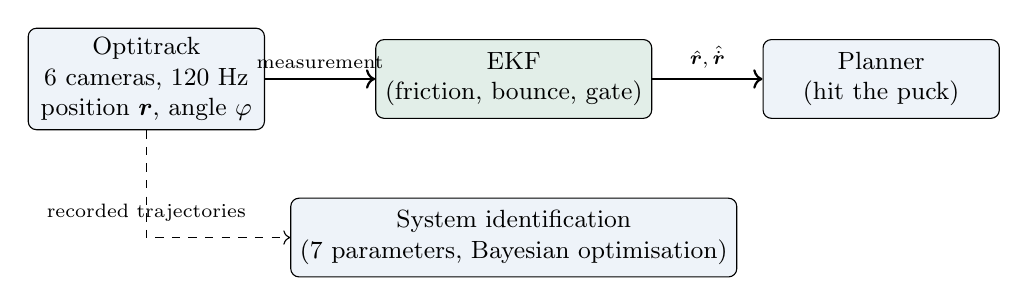
\begin{tikzpicture}[node distance=1.2cm, every node/.style={font=\small},
 box/.style={draw, rounded corners=3pt, minimum width=3.0cm, minimum height=1.0cm, align=center, fill=cblue!8},
 ours/.style={draw, rounded corners=3pt, minimum width=3.0cm, minimum height=1.0cm, align=center, fill=cgreen!14}]
\node[box] (opt) {Optitrack\\6 cameras, 120 Hz\\position $\rr$, angle $\varphi$};
\node[ours, right=1.4cm of opt] (ekf) {EKF\\(friction, bounce, gate)};
\node[box, right=1.4cm of ekf] (plan) {Planner\\(hit the puck)};
\draw[->, thick] (opt) -- node[above]{\scriptsize measurement} (ekf);
\draw[->, thick] (ekf) -- node[above]{\scriptsize $\hat\rr,\hat{\dot\rr}$} (plan);
\node[box, below=1.0cm of ekf, minimum width=5.2cm] (sim) {System identification\\(7 parameters, Bayesian optimisation)};
\draw[->, dashed] (opt.south) |- node[below, pos=0.3]{\scriptsize recorded trajectories} (sim.west);
\end{tikzpicture}
\caption{What the paper does. The green box is the part we use.}
\end{figure}

\begin{idea}[One sentence to remember]
\emph{A tracking filter for a sliding, bouncing object is an ordinary Kalman filter with two
extra pieces of physics, a friction term in the prediction and a bounce rule when the object hits
a wall, plus a rule for what to do when a measurement does not fit.}
\end{idea}

% ============================================================ 3
\section{Glossary}

\begin{center}
\begin{tabularx}{\textwidth}{@{}l X@{}}
\toprule
Term & Meaning \\
\midrule
Puck & The air hockey disc. Slides with very little friction. \\
Mallet & The paddle that the robot holds to hit the puck. \\
Optitrack & Infrared motion-capture cameras that track reflective markers; the paper reports $1$~mm precision. \\
EKF & Extended Kalman filter: a Kalman filter for a nonlinear model, linearised at each step with a Jacobian. \\
Prediction step & Use the model to guess the next state (and its uncertainty) before the new measurement arrives. \\
Update step & Correct the guess with the new measurement. \\
Innovation $\bm y$ & Measurement minus predicted measurement: how much the new data surprised the filter. \\
Innovation covariance $S$ & The filter's own estimate of how big a typical innovation should be. \\
Mahalanobis distance $d$ & $d^2=\bm y^{\mathsf T}S^{-1}\bm y$: the innovation measured in units of its expected size. \\
Gating & Accept a measurement only if its Mahalanobis distance is below a threshold. \\
Restitution $E$ & Fraction of the normal speed kept after a bounce. \\
System identification & Finding the parameters of a model from measured data. \\
Bayesian optimisation (BO) & A way to optimise a function that is expensive to evaluate and has no gradient, by fitting a statistical model to the points tried so far and choosing the next point cleverly. \\
Gaussian process (GP) & The statistical model that BO uses to predict the function and its uncertainty. \\
Acquisition function (EI, PI, UCB) & The rule that picks the next point to try: expected improvement, probability of improvement, upper confidence bound. \\
HEBO & Heteroscedastic evolutionary Bayesian optimisation: a BO variant that copes with noise whose size varies. \\
Null space, redundancy & Robot-arm terms for the extra joint freedom; part of the planning half of the paper that we skip. \\
\bottomrule
\end{tabularx}
\end{center}

% ============================================================ 4
\section{The paper, section by section}

\subsection{Introduction and problem (paper, Sec.~I)}
The authors want a \emph{general-purpose} 7-joint arm to play air hockey almost as well as
task-specific planar robots. They describe the air hockey problem: a table $T$, two goals, a
circular puck with position $\bm r$ and orientation $\varphi$, and two mallets. The puck changes
direction only through a collision with a mallet or a table border. Each player maximises the
number of goals. The authors stress two sources of uncertainty: the uneven airflow through the
holes of the table, and the sensitive, variable collision behaviour.

\subsection{Preliminaries (paper, Sec.~II)}
Part~A recalls robot kinematics (forward kinematics, the Jacobian, the null space of a redundant
arm). Part~B explains \textbf{Bayesian optimisation}: to maximise an unknown function $f(\theta)$ you
(1)~fit a Gaussian process to the values observed so far, which predicts a mean $\mu(\theta)$ and an
uncertainty, and (2)~maximise an \emph{acquisition function} that balances exploring uncertain
regions and exploiting promising ones. Three acquisition functions are named: EI, PI, UCB. We do not
need the details; the idea is ``a smart search without gradients''.

\subsection{Hitting optimisation (paper, Sec.~III)}
This is the robot-motion core of the paper: plan a collision-free path for the mallet made of
straight lines and arcs, then choose joint velocities with a quadratic program that uses the extra
joint freedom (null space) to reach the highest hitting speed within the joint limits, and
optimise the arm's configuration at the hit point. It has nothing to do with estimating a ball, so
I do not explain it further. Its results (Table~II) are computation times of about $130$--$260$~ms
per hit (paper).

\subsection{System identification (paper, Sec.~IV)}
\label{sec:sysid}
The authors build a puck simulator (in Gazebo) with \textbf{seven tunable parameters} (paper,
Table~I), each searched within a range:

\begin{center}
\small
\begin{tabular}{@{}lcc@{}}
\toprule
parameter & min & max \\
\midrule
restitution, long-side rim & 0.5 & 1 \\
restitution, short-side rim & 0.5 & 1 \\
friction coefficient, rim & 0 & 0.5 \\
friction coefficient, table surface & 0 & 0.5 \\
puck spinning & 0 & 0.5 \\
puck linear velocity decay & 0 & 0.01 \\
puck angular velocity decay & 0 & 0.01 \\
\bottomrule
\end{tabular}
\end{center}

The quantity to \textbf{minimise} is the average mismatch between simulated and real recorded
trajectories (paper):
\[
f(\theta)=\mathbb E_{i\sim U[1:N]}\!\left[\frac1T\sum_{t=1}^{T}\|\Delta\bm r_t^{(i)}(\theta)\|_2^2+0.2\,\|\Delta\varphi_t^{(i)}(\theta)\|_\angle^2\right],
\]
where $\Delta\bm r_t^{(i)}=\bm r_t^{(i)}-\hat{\bm r}_t^{(i)}(\theta)$ is the position error at time $t$ on
recorded trajectory $i$ (real minus simulated), $\Delta\varphi$ is the (shortest) angle error, the
weight $0.2$ makes the angle count less than the position, and $U$ is a uniform pick over the $N$
recorded trajectories. In words: \emph{run the simulator with the guess $\theta$, start it from the
same initial state as each real trajectory, and measure how far the simulated puck drifts from the
real one.}

Because Gazebo cannot be differentiated, they use Bayesian optimisation. Two problems arise
(paper): the noise is \emph{heteroscedastic} (its size changes, because collisions make it
non-Gaussian), and the choice of acquisition function is unclear. They adapt \textbf{HEBO} to handle
both, using input and output warping and a multi-objective acquisition (a Pareto solution between
EI, PI and UCB). They run \textbf{200 iterations, with 5 candidate parameter vectors per iteration}
(paper, Sec.~VI-B). HEBO beat the other BO methods they tried, and the result is ``sufficiently good
to be used in a simulation'', but ``there is still some discrepancy between the real trajectory and
the simulated one'', particularly at slow velocities (airflow and surface irregularities).

\subsection{Hardware and the Optitrack measurement (paper, Sec.~V-A)}
Two Kuka iiwa 14 arms, each with an end-effector of $515$~mm with a gas spring and a universal
joint (for safety). \textbf{Six Optitrack Flex 13 cameras, $1920\times1680$ resolution, $120$~Hz,
placed above the table, track markers on the puck and the table, giving $1$~mm tracking precision}
(paper). In simulation, the poses come directly from the simulator (no sensor model at all).

\subsection{The EKF state estimator (paper, Sec.~V-B)}
\label{sec:ekf}
This is the part we study closely. The measurements are the puck's position $\bm r_t$ and
orientation $\varphi_t$. The filter estimates their velocities $\dot{\bm r}_t$ and $\dot\varphi_t$.
The \textbf{transition model} printed in the paper is
\begin{align*}
\bm r_{t+1}&=\bm r_t+\dot{\bm r}_t\,\Delta T+\bm\varepsilon_r,\\
\dot{\bm r}_{t+1}&=\dot{\bm r}_t-\bigl(d\,\dot{\bm r}_t+c(\dot{\bm r}_t)\bigr)\Delta T+\bm\varepsilon_{\dot r},\\
\varphi_{t+1}&=\mathrm{wrap}(\varphi_t+\dot\varphi_t\,\Delta T+\varepsilon_\varphi),\\
\dot\varphi_{t+1}&=\dot\varphi_t+\varepsilon_{\dot\varphi},
\end{align*}
where $\Delta T$ is the time step, each $\varepsilon_k$ is Gaussian noise on that state, $d$ is a
linear \emph{drag} coefficient, and $c(\cdot)$ is the \emph{friction} vector with component
\[
c_i(\dot{\bm r})=\begin{cases}c,&|\dot r_i|>0\\0,&\text{otherwise.}\end{cases}
\]
Line by line: the position moves by velocity times time; the velocity \emph{shrinks} through drag
(proportional to speed) and constant friction; the angle moves by the angular velocity and is
wrapped into $(-\pi,\pi]$; the angular velocity is a random walk.

\begin{eqbox}[The same model in our notation (my rewrite, planar ball without spin)]
State $s=(x,y,v_x,v_y)^{\mathsf T}$, measurement $z=(x,y)^{\mathsf T}$:
\[
\begin{aligned}
\bm r_{k+1}&=\bm r_k+\vv_k\,\Delta T,\\
\vv_{k+1}&=\vv_k-\Bigl(d\,\vv_k+c\,\frac{\vv_k}{\|\vv_k\|}\Bigr)\Delta T,\\
z_k&=H s_k+\text{noise},\quad H=\begin{pmatrix}1&0&0&0\\0&1&0&0\end{pmatrix}.
\end{aligned}
\]
The friction acts \emph{against} the velocity with constant size $c$ (the deceleration $\mu$ of our
simulator is exactly this $c$, and our simulator has $d=0$). Because of the division by
$\|\vv_k\|$ the model is nonlinear in the velocity, which is why the filter is \emph{extended}:
its transition matrix is the Jacobian of this map,
\[
F=\begin{pmatrix}I&\Delta T\,I\\0&I-d\,\Delta T\,I-\dfrac{c\,\Delta T}{\|\vv\|}\bigl(I-\hat{\vv}\hat{\vv}^{\mathsf T}\bigr)\end{pmatrix},\qquad \hat{\vv}=\vv/\|\vv\|.
\]
(The lower-right block follows from differentiating $\vv/\|\vv\|$; it is my derivation.)
\end{eqbox}

\textbf{Prediction and update.} The standard EKF equations (they are not printed in the paper)
are, with $P$ the state covariance, $Q$ the process-noise covariance and $R$ the measurement
covariance:
\[
\begin{aligned}
\text{predict:}\quad & \hat s^-=f(\hat s),\qquad P^-=F P F^{\mathsf T}+Q,\\
\text{update:}\quad & y=z-H\hat s^-,\quad S=HP^-H^{\mathsf T}+R,\quad K=P^-H^{\mathsf T}S^{-1},\\
& \hat s=\hat s^-+K y,\qquad P=(I-KH)P^-.
\end{aligned}
\]
The paper gives \textbf{no numeric values for $Q$, $R$, $d$ or $c$}.

\begin{toy}[Toy example: why the friction term needs a sign]
Take $c=0.5$~m/s$^2$ and $\Delta T=1/60$~s (so $c\,\Delta T=0.0083$~m/s). A ball moving at
$\dot r=-2$~m/s (towards negative $x$):
\begin{itemize}
\item \textbf{Literal reading of the paper's formula} ($c_i=c$ whenever $|\dot r_i|>0$, subtracted as
printed): $\dot r_{next}=-2-0.0083=-2.0083$. The ball \emph{speeds up}.
\item \textbf{Correct physics} (friction opposes the motion, so $c\,\mathrm{sign}(\dot r)$ is
subtracted): $\dot r_{next}=-2+0.0083=-1.9917$. The ball slows down.
\end{itemize}
As printed, the formula is only right for positive velocities. I believe it is a notation slip and
that the sign is meant; our version above uses $\vv/\|\vv\|$.
\end{toy}

\subsubsection{The collision model and the covariance (paper, Sec.~V-B)}
\label{sec:cov}
\textbf{Collision model.} The paper says: ``After each prediction step, we apply the collision model
from [1]'' (Partridge and Spong, 2000: a model of a planar body sliding with impacts and friction).
\textbf{The paper does not print the collision equations, and I have not read [1]}, so I cannot
say exactly what the authors implemented. For our simpler ball (no spin, frictionless wall), the
natural collision model is the reflection with restitution $E$ that our simulator uses. At the
$60$~Hz rate of the filter the ball can pass a wall \emph{inside} one time step, so the prediction
must reflect the overshoot too. If $L$ is the limit for the ball's centre and the straight-line
prediction is $x_{pred}=x+v\,\Delta T>L$, the reflected prediction (my derivation) is
\[
x^+=L-E\,(x_{pred}-L),\qquad v^+=-E\,v,
\]
with Jacobian entries $\partial x^+/\partial x=-E$, $\partial x^+/\partial v=-E\,\Delta T$,
$\partial v^+/\partial v=-E$.

\begin{toy}[Toy example: a bounce inside one time step]
$L=0.97$~m, ball at $x=0.95$~m moving at $v=+3$~m/s, $E=0.8$, $\Delta T=1/60$~s. The straight-line
prediction is $x_{pred}=0.95+0.05=1.00$~m, i.e.\ $3$~cm beyond the wall. The reflected prediction is
$x^+=0.97-0.8\cdot0.03=0.946$~m and $v^+=-2.4$~m/s. A filter without a wall model is wrong by
$1.000-0.946=5.4$~cm in position and by $3-(-2.4)=\mathbf{5.4}$~m/s in velocity (it even has the
wrong sign).
\end{toy}

\textbf{Covariance at a collision.} ``Every time a collision happens, we don't update the
covariance matrix, as it is hard to model the bounce uncertainty'' (paper). So the filter changes
the \emph{state} through the bounce rule but leaves the uncertainty $P$ as if nothing had happened.
(The paper does not say whether this means $F$ is replaced by the identity for $P$ or the whole
$P$ prediction is skipped; I read it as: $P$ is not changed by the bounce.)

\subsubsection{Gating and the track reset (paper, Sec.~V-B)}
\label{sec:gate}
``We use an ellipsoidal gating procedure for the Optitrack measure. To compute the gate, we use the
innovation covariance matrix and a gate probability of 90\%, i.e., we reject the 10\% of the possible
measurement which belongs to the tail of our estimated distribution.'' Then the key reasoning: since
Optitrack is very unlikely to produce outliers, \textbf{an outlier is interpreted as an unexpected
collision}; so instead of rejecting the measurement, they \textbf{reset the track with the new
measurement and set the state covariance to the initial one, the identity matrix}.

In symbols: compute $d^2=y^{\mathsf T}S^{-1}y$. If $d^2$ exceeds the $90\%$ quantile of a
$\chi^2$ distribution with as many degrees of freedom as the measurement has (for a 2D position:
$d^2>4.605$, i.e.\ $d>2.146$), declare an outlier and reset.

\begin{toy}[Toy example: what a gate does]
Suppose the innovation covariance is $S=\mathrm{diag}(1,1)$~cm$^2$. For a 2D position the gate
limits are $d^2<4.605$ (90\%) or $d^2<9.210$ (99\%).
\begin{itemize}
\item Innovation $(2.0,\,0.5)$~cm: $d^2=4.25$, inside both gates, accepted.
\item Innovation $(2.5,\,1.5)$~cm: $d^2=8.50$, outside the 90\% gate (reset!), inside the 99\% gate.
\end{itemize}
\end{toy}

\subsubsection{The agent strategy (paper, Sec.~V-C) and the evaluation (Sec.~VI)}
The remaining part is a finite state machine with the tactics (Init, Home, Ready, Smash, Repel,
Prepare, Cut) and the hitting results (Fig.~5, Table~II). I skip both. The paper evaluates the
\emph{hitting optimisation} on a grid of 180 puck positions and the \emph{system identification}
through learning curves; it \textbf{does not evaluate the Kalman filter at all} (``the result of the
Kalman filter'' is shown in a video).

\subsection{Conclusion (paper, Sec.~VII)}
They claim a general-purpose arm can hit strongly, that the optimisation runs in real time, and
that Bayesian optimisation offers a simple way to tune a simulator with black-box access only.
Future work: study BO for non-differentiable collisions, include dynamics in the optimisation, and
test the full game on the real system.

% ============================================================ 5
\section{Numbers worth remembering}

\begin{center}
\small
\begin{tabularx}{\textwidth}{@{}X l@{}}
\toprule
Item & Value \\
\midrule
Table size & $216\times122$~cm \textbf{(paper)} \\
Optitrack & 6 cameras, $120$~Hz, $1$~mm precision \textbf{(paper)} \\
Gate probability & $90\%$ (reject $10\%$ tail) \textbf{(paper)} \\
Covariance after a reset & identity matrix \textbf{(paper)} \\
Restitution search range & $0.5$ to $1$ \textbf{(paper, Table~I)} \\
System-identification budget & 200 iterations, 5 candidates each \textbf{(paper)} \\
Hit-optimisation time & $130$--$260$~ms mean \textbf{(paper, Table~II)} \\
Filter noise $Q$, $R$, friction $c$, drag $d$ & \textbf{not given} \\
Filter accuracy & \textbf{not given} \\
\bottomrule
\end{tabularx}
\end{center}

% ============================================================ 6
\section{Critical reading (my comments)}

\begin{warn}[1. The estimator is not evaluated]
There is no table, no plot and no number for the EKF's position or velocity error. A reader
cannot know how good it is. This paper tells us \emph{what} to build but not \emph{how well it
works}; we must measure that ourselves on our dataset.
\end{warn}

\begin{warn}[2. The friction term as printed has no sign]
See the toy example. It is probably notation, but any implementation must use
$c\,\vv/\|\vv\|$. A related numerical issue (my own point): near rest a constant friction can push the
speed through zero and make the estimate chatter, so the friction must be switched off, or clamped,
when $\|\vv\|\,\Delta T$ is smaller than $c\,\Delta T^2$.
\end{warn}

\begin{warn}[3. A 90\% gate rejects 10\% of good measurements]
If the filter is correct, the Mahalanobis distance of a \emph{valid} measurement exceeds the 90\%
gate in exactly $10\%$ of the frames, by definition. At $60$~Hz that is $6$ frames per second. If
every gate failure triggers a track reset with an identity covariance, the filter would restart
about six times per second, throwing away its velocity estimate. Either the filter's $S$ is much
larger than the real noise (so that the gate rarely fires, but then the gate does not do its job),
or the reset happens only under extra conditions that the paper does not describe. A
conventional choice is a $99\%$ gate ($d^2<9.21$ for 2D). I would not copy the 90\% value.
\end{warn}

\begin{warn}[4. Not touching $P$ at a bounce makes the filter overconfident]
Near a wall the outcome of one time step can be \emph{two-valued}: the ball either reaches the wall
inside the step and bounces, or it does not. In a toy with three equally likely positions $1$~cm
apart (wall at $0.97$~m, $v=3$~m/s, $E=0.8$) the velocities after the step are $+3.0$, $-2.4$ and
$-2.4$~m/s: a mean of $-0.6$ and a spread of $2.55$~m/s, while a filter that applies the bounce
rule to its mean and leaves $P$ unchanged keeps a velocity $\sigma$ of about $0.2$~m/s. A Monte
Carlo run ($1$~cm and $0.2$~m/s uncertainty) gives a true spread of $2.0$~m/s when the predicted
position is about $1$~cm from the wall. Because the gain depends on $\sigma$, the overconfident
filter corrects its velocity about $11$ times more slowly after the bounce ($K_v=4.9$ against $56$
for an honest $\sigma_v=2.5$~m/s in a 1D calculation). The deeper issue is that a single Gaussian
cannot describe a two-valued outcome. Paper 05 (the ``salted'' Kalman filter) inflates the
covariance at a bounce, and papers 01 and 16 keep several motion hypotheses.
\end{warn}

\begin{warn}[5. ``Outlier means collision'' is a hypothesis, not a fact]
With Optitrack, outliers are rare, so the argument is reasonable. With our noisy, delayed and
sometimes lost camera measurements, an outlier may be a depth outlier, a stale value, or a real
unmodelled bounce. A silent-hold dropout (paper 11) repeats an old position, which the gate would
soon call an outlier, and then the filter would \emph{reset onto the stale value}. The combination
of this paper's gating rule with our dropout modes needs a test.
\end{warn}

\begin{warn}[6. Offline identification, fixed parameters]
The physical parameters are tuned once from recorded data and then fixed. In our dataset the
friction $\mu$ and the restitution $E$ change from launch to launch, so any fixed nominal values
are wrong in almost every launch. This is the motivation for estimating them online
(gray-box filters, paper 03).
\end{warn}

% ============================================================ 7
\section{What this means for our chapter}

\begin{ours}[1. Our first real estimator: ``EKF-19'']
State $(x,y,v_x,v_y)$, measurement $(x,y)$, prediction with friction $c\,\vv/\|\vv\|$, reflection with
restitution $E$ at the walls (in the 4 walls of our arena), standard EKF update. It runs at the
frame rate and uses the capture time stamp of each measurement (paper 11's delay handling). With a
\textbf{flagged} dropout it simply predicts without an update. We then compare it with the plainer
baselines (finite differences, constant-velocity Kalman filter) on the same $500$ launches.
\end{ours}

\begin{ours}[2. Where its numbers come from]
$Q$ and $R$ are not given by the paper. We can tune them (and a nominal $c$ and $E$) offline with a
black-box optimiser on part of our dataset, minimising the \emph{prediction error} as the loss,
exactly like the paper's system-identification loop but for the filter instead of the simulator.
Plain starting points: $R$ from the camera ($\sim$ a pixel, $7$~mm), nominal $c=0.85$~m/s$^2$ and
$E=0.725$ (middle of our sampled ranges).
\end{ours}

\begin{ours}[3. Decisions that I would take from the paper, and the ones I would change]
\begin{itemize}
\item \textbf{Keep:} the friction term (with a sign), the bounce rule, the gate idea.
\item \textbf{Change:} use a $99\%$ gate (not $90\%$); treat a gate failure as a \emph{flag}, and test
the ``reset'' rule against ``skip the measurement'' on our data.
\item \textbf{Improve later:} inflate $P$ at a bounce (paper 05), estimate $c$ and $E$ online
(paper 03), switch between regimes (papers 01 and 16).
\end{itemize}
\end{ours}

\begin{ours}[4. The restitution range]
The paper searches $E\in[0.5,\,1]$ for a real air hockey table. Our $E\in[0.5,\,0.95]$ is consistent
with that, so it is not only my guess any more. Their friction ``coefficients'' ($0$--$0.5$) are
dimensionless and not comparable with our deceleration $\mu$ in m/s$^2$ (ours corresponds to a
friction coefficient of $\mu/g=0.02$--$0.15$).
\end{ours}

\begin{toy}[Toy example: how much does knowing the friction matter over a gap?]
The camera loses the ball for $0.2$~s (flagged), and the filter predicts. True deceleration
$0.5$~m/s$^2$. A constant-velocity prediction ($c=0$) is off by $\tfrac12\cdot0.5\cdot0.2^2=10$~mm. A
friction-aware prediction with a \emph{wrong} nominal $c=0.9$ is off by
$\tfrac12\cdot|0.9-0.5|\cdot0.2^2=8$~mm. So over short gaps the exact friction hardly matters; what
matters much more is whether a \emph{bounce} happens inside the gap (the toy above gives errors of
several centimetres and a wrong velocity sign).
\end{toy}

\begin{eqbox}[Decisions for you]
(1)~Gate: do you accept the $99\%$ gate and testing both ``reset'' and ``skip the measurement''?
(2)~Nominal $c$ and $E$: use the middle of our ranges first and tune offline later?
(3)~Should the first baseline set include the EKF-19 \emph{with} an oracle (it is told the true
$\mu$ and $E$ of each launch) as an upper bound, in addition to the realistic nominal one?
\end{eqbox}

% ============================================================ 8
\section{Test yourself}

\begin{enumerate}
\item Write the prediction step of the paper's EKF for a puck without spin. What is the role of the
friction term and of the drag term?
\item Why does the friction term need $\vv/\|\vv\|$ and not just a constant?
\item What does the innovation covariance $S$ represent, and what is the Mahalanobis distance?
\item A valid measurement is tested against a 90\% gate. How often does it fail the test? Why is
this a problem for the paper's reset rule?
\item Why does leaving $P$ unchanged at a bounce make the filter overconfident?
\item A ball at $x=0.95$~m with $v=2$~m/s, wall at $0.97$~m, $E=0.8$, $\Delta T=1/60$~s. Compute
the reflected prediction. (Answer: $x_{pred}=0.9833$, overshoot $0.0133$, $x^+=0.9593$,
$v^+=-1.6$~m/s.)
\item What does the paper's system-identification loss measure, and why is Bayesian optimisation
needed?
\item Which parts of this paper are \emph{not} usable for our chapter, and why?
\end{enumerate}

\appendix
\section{Map of the paper}
\begin{center}
\small
\begin{tabularx}{\textwidth}{@{}l X@{}}
\toprule
Paper part & Content and where it is in this guide \\
\midrule
Sec.~I & Problem statement, related work (Sec.~4.1) \\
Sec.~II & Kinematics and Bayesian optimisation (Sec.~4.2) \\
Sec.~III & Hitting optimisation, QP/NLP/AQP (Sec.~4.3, skipped) \\
Sec.~IV & System identification, Table~I, loss (Sec.~4.4) \\
Sec.~V-A & Hardware, Optitrack (Sec.~4.5) \\
Sec.~V-B & \textbf{EKF, collision, covariance, gate} (Sec.~4.6) \\
Sec.~V-C & State machine (Sec.~4.6.3, skipped) \\
Sec.~VI & Evaluation (Sec.~4.6.3) \\
Sec.~VII & Conclusion (Sec.~4.7) \\
\bottomrule
\end{tabularx}
\end{center}

\end{document}
